%%%%%%%%%%%%%%%%%%%%%%%%%%%%%%%%%%%%%%%%%
% Modified Template for AI Fingerspelling Recognition Project
% Based on Dreuw & Deselaer's Poster
% LaTeX Template
% Version 2.1 (January 5, 2024)
%%%%%%%%%%%%%%%%%%%%%%%%%%%%%%%%%%%%%%%%%
%
% This template originates from:
% https://www.LaTeXTemplates.com
%
% Authors:
% Vel (vel@latextemplates.com)
% Philippe Dreuw and Thomas Deselaers (https://github.com/deselaers/latex-beamerposter)
%
% License:
% CC BY-NC-SA 4.0 (https://creativecommons.org/licenses/by-nc-sa/4.0/)
%
%%%%%%%%%%%%%%%%%%%%%%%%%%%%%%%%%%%%%%%%%

%----------------------------------------------------------------------------------------
%	PACKAGES AND OTHER DOCUMENT CONFIGURATIONS
%----------------------------------------------------------------------------------------

\documentclass{beamer} % Use the beamer base class

\usepackage[
	orientation=landscape, % Portrait orientation
	size=a1, % Paper size
	scale=1, % Scale, it's important to adjust this so your content fits nicely in the template
]{beamerposter} % Use the beamerposter package to create the layout

\usetheme{I6pd2} % Use the I6pd2 theme supplied with this template

\usepackage{changepage} % Required for temporarily indenting text blocks

\usepackage{amsmath,amsthm,amssymb,latexsym} % For including math equations, theorems, symbols, etc

\usepackage{gfsdidot} % Use the GFS Didot font

\usepackage{booktabs} % Top and bottom rules for tables

\usepackage{subcaption} % Required for subfigures

\usepackage[export]{adjustbox} % Required for image alignment

\usepackage{natbib} % Required for bibliography

\graphicspath{{Figures/}} % Location of figure images

%----------------------------------------------------------------------------------------
%	TITLE SECTION
%----------------------------------------------------------------------------------------

\title{\LARGE AI-Based ASL Fingerspelling Recognition Using the Google Kaggle Dataset for Automated Kiosk Transactions}  % Poster title

\subtitle{A Literature Review and Project Application}

\author{Jamie Pinnington\texorpdfstring{\textsuperscript{1,2}}{1,2}, Amina Souag\texorpdfstring{\textsuperscript{2,3}}{2,3}, Hannan Azhar\texorpdfstring{\textsuperscript{2,3}}{2,3}}  % Author(s)

\institute{\textsuperscript{1}Computer Science, \textsuperscript{2}Canterbury Christ Church University, \textsuperscript{3}School of Engineering, Technology and Design}  % Institution(s)

%----------------------------------------------------------------------------------------
%	FOOTER TEXT
%----------------------------------------------------------------------------------------

\newcommand{\leftfoot}{https:jamie-pinnington.co.uk} % Left footer text

\newcommand{\rightfoot}{JP878@canterbury.ac.uk} % Right footer text

%\setbeamertemplate{footline}{} % Uncomment this line to hide the footer

%----------------------------------------------------------------------------------------

\begin{document}

\setbeamertemplate{caption}[numbered]

\begin{frame}[t] % The whole poster is enclosed in one beamer frame, the [t] parameter aligns everything to the top

	\begin{columns}[t] % Begin multi-column layout, the [t] parameter aligns each column's content to the top

		\begin{column}{0.005\textwidth}\end{column} % Empty column for horizontal whitespace

		\begin{column}{0.3\textwidth} % Start the first content column

			%----------------------------------------------------------------------------------------
			%	Introduction
			%----------------------------------------------------------------------------------------

			\begin{block}{Introduction}
				\begin{itemize}
					\item According to \cite{ethnologueAmericanSignLanguage2023,mitchellHowManyPeople2006}, there are at least 1 million if not more American Sign Language (ASL) users in the United States alone who are a part of the Deaf and Hard of Hearing (DHH) community.

					\item Fingerspelling is a critical component of ASL and other sign languages, and is used to spell out words, names, and proper nouns that lack direct signs.

					\item Current recognition solutions for ASL, don't include fingerspelling, and typically don't work effectively in the real world.

					      % Reduce space before the minipage
					      \vspace{-\baselineskip}
					      \begin{minipage}{\textwidth}
						      \begin{minipage}{.75\textwidth}
							      \vspace{0pt}
							      \item Legal concerns from the largest and most used ChicagoWild/+ dataset, have made it difficult for commercial application.

							      \item A new dataset released on Kaggle by Google \citep{kaggleAslFinger} has provided a new opportunity to explore how applying AI could improve, assist, and provide options to the lives of the DHH and the wider community?
						      \end{minipage}%
						      \begin{minipage}{.2\textwidth}
							      \vspace{0pt}
							      
\includegraphics[width=2.5in]{qr_paper_v1.png}
						      \end{minipage}
					      \end{minipage}
					      % Adjust space after the minipage if needed
					      \vspace{-\baselineskip}
				\end{itemize}
			\end{block}

			%----------------------------------------------------------------------------------------
			%	Methodology
			%----------------------------------------------------------------------------------------


			\begin{block}{Methodology}
				\begin{figure}
					\centering
					\begin{subfigure}[t]{0.24\linewidth}
						
\includegraphics[width=\linewidth,valign=t]{ieee_xplore.png}
					\end{subfigure}
					\hfill % Add horizontal space
					\begin{subfigure}[t]{0.24\linewidth}
						
\includegraphics[width=\linewidth,valign=t]{acm_4c_grad_pos.png}
					\end{subfigure}
					\hfill % Add horizontal space
					\begin{subfigure}[t]{0.24\linewidth}
						
\includegraphics[width=\linewidth,valign=t]{ScienceDirect-Librarian-Promo-Toolkit_Logo.png}
					\end{subfigure}
					\hfill % Add horizontal space
					\begin{subfigure}[t]{0.24\linewidth}
						
\includegraphics[width=\linewidth,valign=t]{scholar_logo_64dp.png}
					\end{subfigure}
				\end{figure}
				\begin{minipage}{0.48\linewidth}
					Literature Identification
					\begin{enumerate}
						\item Conducted research across four academic databases.
						\item Focused on papers published within the last 5 years (2018-2023).
						\item Limited to peer-reviewed journal articles, conference papers, and high-quality theses.
						\item Search conducted in English only.
						\item Search period: November to December 2023.
						\item Search terms such as "ASL fingerspelling", "ASL recognition in real-time", "Deep learning for ASL fingerspelling".
					\end{enumerate}
				\end{minipage}
				\hfill % Add horizontal space
				\begin{minipage}{0.48\linewidth}
					Literature Evaluation
					\begin{enumerate}
						\item Abstract → relevance → full reading of selected papers
						\item Summarization and analysis of findings in a table
						\item \alert {Inclusion} Relevance to research questions
						\item Specific focus on ASL fingerspelling
						\item Use of machine learning (ML) models in sign language interpretation
						\item Utilization of recognized datasets relevant to ASL recognition
						\item Clear methodology, defined objectives, data analysis
						\item High citation counts preference
						\item \alert {Excluded} Editorials, opinion pieces, and non-peer-reviewed articles
					\end{enumerate}
				\end{minipage}
			\end{block}

			%----------------------------------------------------------------------------------------
			%	Results: Figure
			%----------------------------------------------------------------------------------------

			\begin{block}{Results: Figure}
				\setcounter{figure}{0}
				\begin{minipage}{\linewidth}
					\begin{figure}
						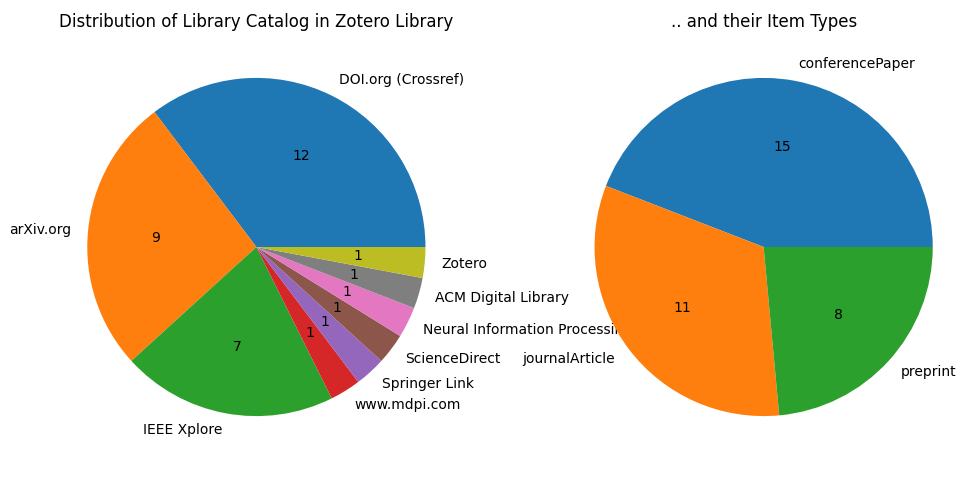
\includegraphics[width=\linewidth]{Figure_1.png}
						\caption{Distribution of Library Catalog and Item Type (2018-2023)}
					\end{figure}
				\end{minipage}
				%\\ % Add a line break here
				%\begin{minipage}{\linewidth} cannot fit this?
				%	\begin{figure}
				%		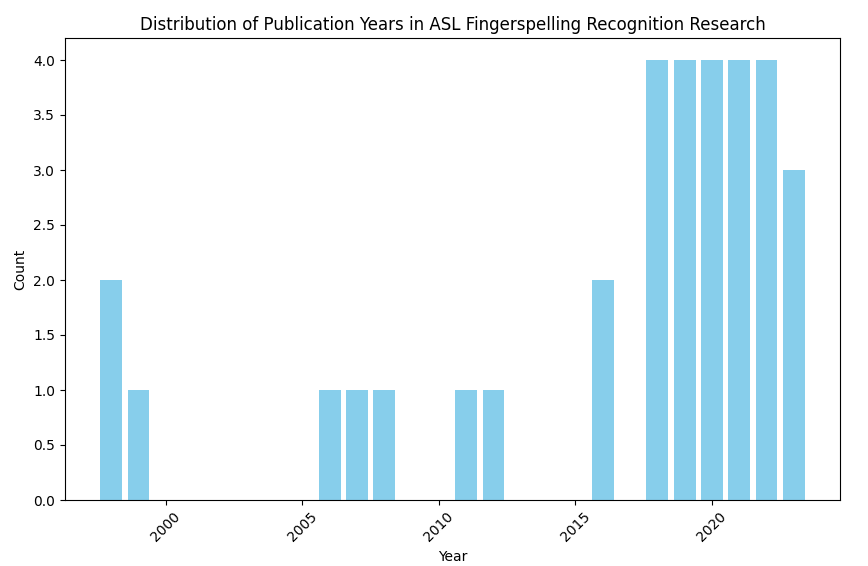
\includegraphics[width=\linewidth]{Figure_2.png}
				%	\end{figure}
				%\end{minipage}
			\end{block}


			%------------------------------------------------

		\end{column} % End of the first column

		\begin{column}{0.005\textwidth}\end{column} % Empty column for horizontal whitespace

		\begin{column}{0.3\textwidth}

			%----------------------------------------------------------------------------------------
			%	Results: Table
			%----------------------------------------------------------------------------------------


			\begin{block}{Results: Table}
				\begin{footnotesize}
					\begin{table}[H]
						\begin{tabular}{p{0.15\textwidth} p{0.65\textwidth} p{0.1\textwidth}}
							\toprule
							Model                         & Key Insights and Performance                                                                                   & Citation                                           \\
							\midrule

							RNN, LSTM, Attention          & Recognition and translation of ASL glosses; GRR: 86\%, GER: 23\%. Challenges in real-time recognition.         & \cite{skumarTimeSeriesNeural2018}                  \\
							CNN, SSD, FCN                 & High accuracy in vision-based translation; Accuracy: 92.21\%. Robustness in ASL recognition.                   & \cite{abiyevReconstructionConvolutionalNeural2020} \\
							Transformers, CTC             & State-of-the-art results in ASL recognition; WER, BLEU-4 scores. Translation challenges addressed.             & \cite{cihancamgozSignLanguageTransformers2020}     \\
							ResNet, Bi-LSTM               & Recognition using optical flow; Letter accuracy: 57\%. Focus on 'wild' conditions and occlusions.              & \cite{kabadeAmericanSignLanguage2023}              \\
							2D/3D-CNN, Bi-LSTM            & Superior detection in diverse environments; AP@IoU: 0.495, MSA: 0.386. Fine-grained handshapes analysis.       & \cite{shiFingerspellingDetectionAmerican2021}      \\
							Fine-Grained Visual Attention & Improved recognition with Transformer model; Letter Accuracy: 46.96\% (dev). Addressing video data challenges. & \cite{gajurelFineGrainedVisualAttention2021}       \\

							\bottomrule
						\end{tabular}
						\caption{Extremely Condensed Summary of ASL Fingerspelling Recognition Models (2018-2023)}
					\end{table}
				\end{footnotesize}
			\end{block}

			%----------------------------------------------------------------------------------------
			%	Discussion
			%----------------------------------------------------------------------------------------

			\begin{block}{Discussion}
				\begin{figure}
					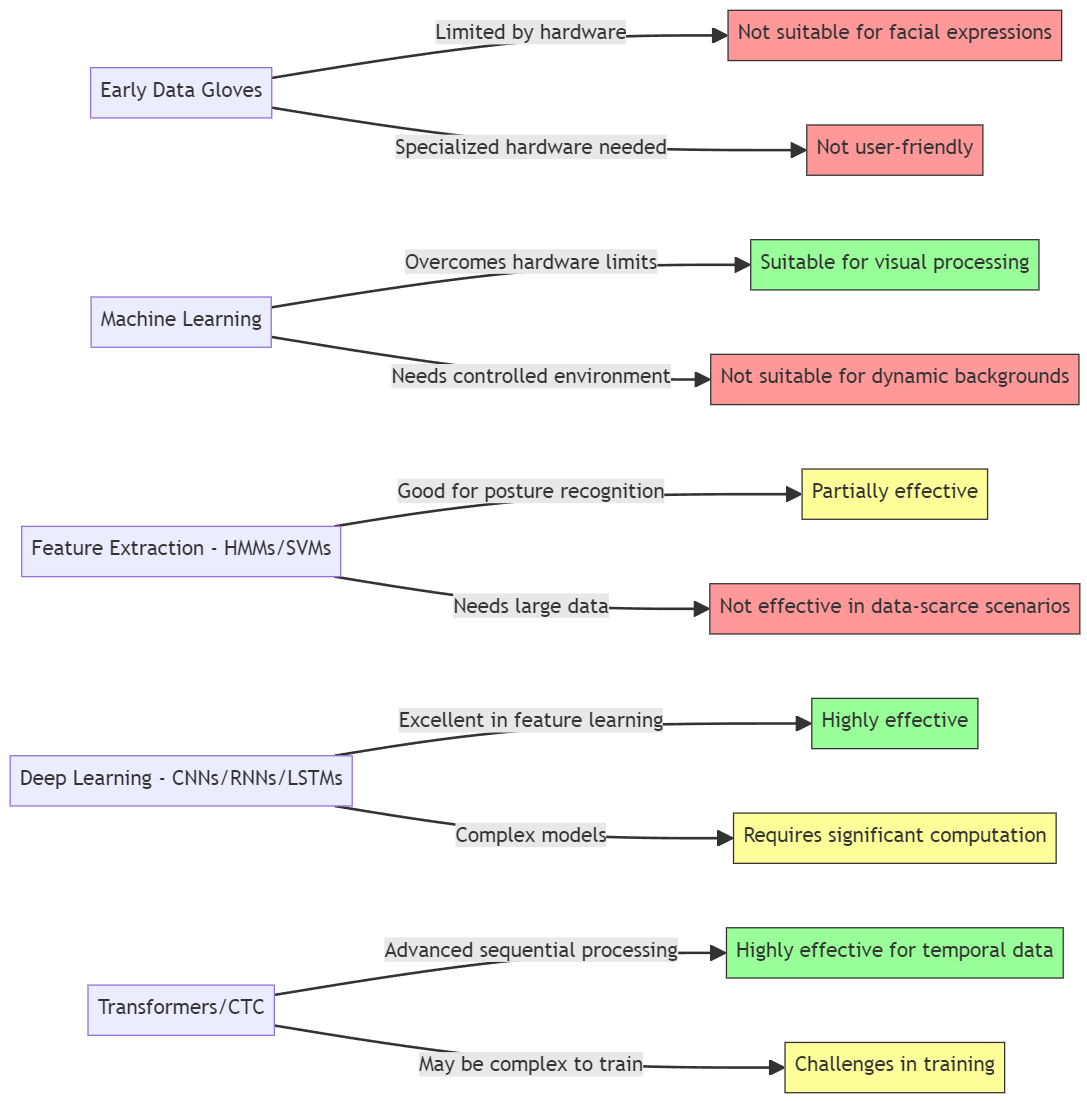
\includegraphics[width=0.95\linewidth]{mermaid-diagram-discussion.png}
					\caption{Generalized Overview of Data Analysis of Results (2018-2023)}
				\end{figure}
			\end{block}

			%----------------------------------------------------------------------------------------
			%	REFERENCES
			%----------------------------------------------------------------------------------------

			\begin{block}{References}
				\fontsize{6}{10}\selectfont
				\vspace{-1ex} % Pull up slightly
				\bibliographystyle{elsarticle-harv}
				\bibliography{../latex/library}
			\end{block}

			%----------------------------------------------------------------------------------------

		\end{column}

		\begin{column}{0.005\textwidth}\end{column} % Empty column for horizontal whitespace

		\begin{column}{0.3\textwidth} % Start the second content column

			%----------------------------------------------------------------------------------------
			%	Graphics and Images Juice
			%----------------------------------------------------------------------------------------

			\begin{block}{Technology and Tools Overview}
				\begin{figure}
					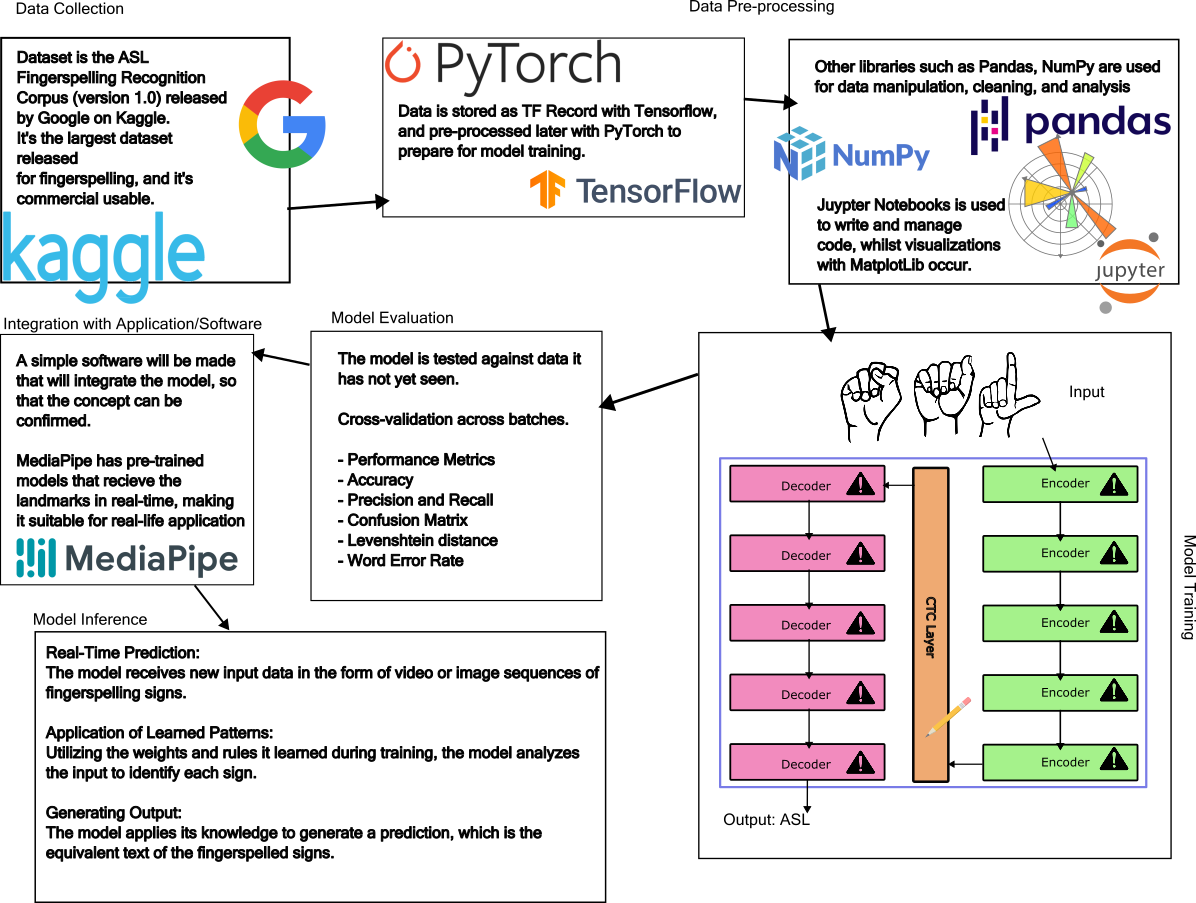
\includegraphics[width=\linewidth]{drawing.png}
					\caption{Technology and Tools Overview}
				\end{figure}
			\end{block}

			%----------------------------------------------------------------------------------------
			%	CONCLUSIONS
			%----------------------------------------------------------------------------------------

			\begin{block}{Conclusions}
				\begin{minipage}{0.75\linewidth}
					\begin{enumerate}
						\item CNNs, RNNs, LSTMs, and their variants are not sufficient for ASL fingerspelling recognition.
						\item Real-world challenges, including rapid signing, varied hand orientations, and diverse environmental conditions, pose substantial difficulties for current models.
						\item Techniques such as data augmentation, transfer learning, and the use of pre-trained models are critical in overcoming these obstacles.
						\item State-of-the-art Models are variants of Transformer.
					\end{enumerate}
					\alert{Model}: The proposed model architecture includes Transformer/Squeezeformer + CTC + Multi-headed Attention + Beam Search.
				\end{minipage}
				\hfill
				\begin{minipage}{0.24\linewidth}
					\begin{figure}
						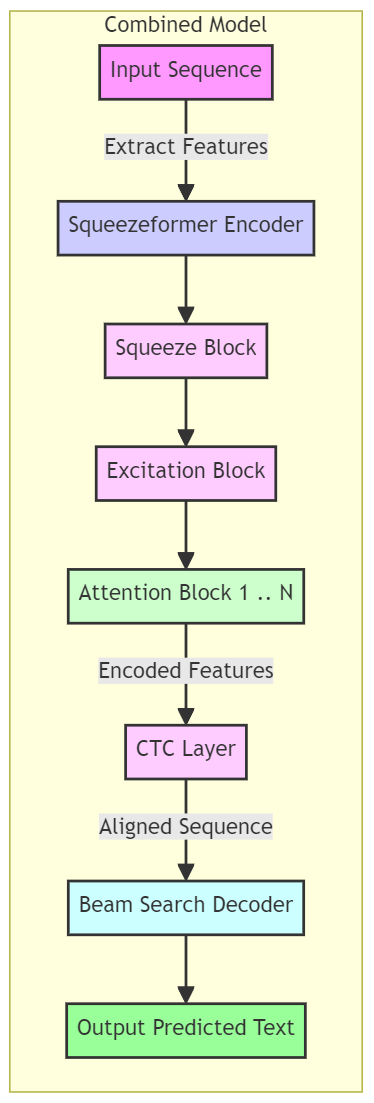
\includegraphics[width=2in]{mermaid-diagram-conclusion.png}
					\end{figure}
				\end{minipage}
			\end{block}

			%----------------------------------------------------------------------------------------
			%	CONTACT INFORMATION
			%----------------------------------------------------------------------------------------

			\setbeamercolor{block title}{fg=black, bg=taorange} % Change the block title color

			\begin{block}{Contact Information}
				\begin{figure}
					\begin{subfigure}[t]{0.25\linewidth}
						\centering
						
\includegraphics[width=1.5in,valign=t]{qr_online_v6.png}
					\end{subfigure}
					\begin{subfigure}[t]{0.45\linewidth}
						\begin{itemize}
							\item Web: \href{https://www.jamie-pinnington.co.uk}{www.jamie-pinnington.co.uk}
							\item Email: \href{mailto:JP878@canterbury.ac.uk}{JP878@canterbury.ac.uk}
							\item Phone: +(44) 07984066009
						\end{itemize}
					\end{subfigure}
					\begin{subfigure}[t]{0.25\linewidth}
						\centering
						
\includegraphics[width=1.5in,valign=t]{qr_linked_v5.png}
					\end{subfigure}
				\end{figure}
			\end{block}

			%----------------------------------------------------------------------------------------
		\end{column} % End of the second column

		\begin{column}{0.005\textwidth}\end{column} % Empty column for horizontal whitespace

	\end{columns} % End of all the columns in the poster

\end{frame} % End of the enclosing frame

%----------------------------------------------------------------------------------------

\end{document}
